% !TeX program = lualatex
% !TeX encoding = utf8
% !TeX spellcheck = uk_UA

\documentclass[]{beamer}
\usetheme{PlasmaPhysics}
\usepackage{PlasmaPhysics}
\usetikzlibrary{shadings}

%\NewDocumentCommand{\E}{}{\vec{E}}
%\NewDocumentCommand{\B}{}{\vec{B}}
%\NewDocumentCommand{\J}{}{\vec{j}}
%\NewDocumentCommand{\V}{}{\vec{v}}
%\NewDocumentCommand{\wk}{}{\vec{k}}
%
%\NewDocumentCommand{\divg}{m}{\vec{\nabla}\cdot{#1}}
%\NewDocumentCommand{\rot}{m}{\vec{\nabla}\times{#1}}
%\NewDocumentCommand{\grad}{m}{\vec{\nabla}#1}
%\NewDocumentCommand{\vecdot}{mm}{\left[#1\times#2\right]}
%\NewDocumentCommand{\scdot}{mm}{\left(#1\cdot#2\right)}
%\NewDocumentCommand{\dt}{m}{\frac{\partial #1}{\partial t}}
%\NewDocumentCommand{\ddt}{m}{\frac{\partial^2 #1}{\partial t^2}}

\usepackage{subcaption}
\usepackage{mathtools}
\setlength{\abovedisplayskip}{3pt}
\setlength{\belowdisplayskip}{3pt}
\usetikzlibrary{decorations.pathreplacing}
\newtcolorbox{mysidebyside}[1][]{
    notitle, sidebyside, blanker,
    sidebyside align=center seam,
    halign=center,
    lefthand width=.5\textwidth,
    #1
}



\graphicspath{{pictures/}}
\title[Лекції з фізики плазми]{\bfseries\huge Магнітогідродинамічні хвилі в плазмі}
\subtitle{\bfseries Лекції з фізики плазми}
\author{Пономаренко С. М.}
\date{}
% https://www.youtube.com/watch?v=zv9Y7YmHyBk
\def\stext#1{\text{
        \makebox[0pt]{
            \tikz[baseline] {\node[text width=50pt, align=center, execute at begin node=\setlength{\baselineskip}{-0.5ex}, blue] {#1};}
        }
}}


\begin{document}




%===============================================================================
\usebackgroundtemplate{
	\tikz\node[opacity=0.1]{\includegraphics[width=\paperwidth,height=\paperheight]{background}};%
}


\begin{frame}
	\thispagestyle{empty}
	\titlepage
\end{frame}

%% --------------------------------------------------------
\section{Вступ}
%% --------------------------------------------------------

% ============================== Слайд ## ===================================
\begin{frame}{Коливальні та хвильові процеси в плазмі}{Преамбула}
	\begin{block}{}\justifying\footnotesize
		Коливальні процеси в плазмі пов'язані з одночасною зміною цілої низки величин, які залежать одна від одної.

		\medskip

		Якщо в плазмі \alert{коливаються напруженості електричного} і \alert{магнітного полів}, то вони збуджують \alert{періодичні струми}. Струм, взаємодіючи з магнітним полем, викликає лоренцову (пондеромоторну) силу, яка приводить плазму в рух. Тому кожен коливальний процес у плазмі супроводжується \alert{періодично зміною швидкості руху самої плазми}, що зі свого боку призводить до \alert{коливань тиску}. Тобто, \alert{коливання плазми є одночасно електромагнітними і гідродинамічними}.

		\medskip

		В окремих випадках основне значення можуть мати зміни тих чи інших величин, і тому наближено можна говорити про \alert{електростатичні}, \alert{електромагнітні}, \alert{магнітогідродинамічні}, \alert{звукові} коливання плазми. Однак потрібно мати на увазі, що такий поділ не універсальний. У низці випадків різні типи коливань переплутуються, і виникає процес, у якому однаково істотні зміни всіх величин, що характеризують плазму.

	\end{block}
\end{frame}
% ===========================================================================

%% --------------------------------------------------------
\section{Магнітогідродинамічні хвилі}
%% --------------------------------------------------------
% ============================== Слайд ## ===================================
\begin{frame}{Звуквові хвилі}{}
	\begin{block}{}\justifying
		Фундаментальний тип хвильового руху, що існує в стисливій непровідній рідині, --- це поздовжні звукові хвилі. Для цих хвиль зміни тиску $p$ і концентрації $n$, пов'язані зі стисненнями і розрідженнями рідини, підкоряються рівнянню адіабати. Градієнт тиску:
		\begin{equation*}
			\grad{p} = \gamma\frac{p}{n}\grad{n} = c_s^2 \grad{(Mn)},
		\end{equation*}
		де $c_s$ ---  швидкість поширення звуку (адіабатична швидкість звука). Звукова хвиля в плазмі --- поширення областей стиснення і розрідження, пов'язані з поздовжнім рухом іонів.

	\end{block}
\end{frame}
% ===========================================================================

% ============================== Слайд ## ===================================
\begin{frame}{Магнітогідродинамічні хвилі}{}
	\begin{block}{}
		У плазмі в магнітному полі, можливі й інші види хвильового руху:

		\begin{enumerate}
			\item іонний звук;
			\item магнітний звук;
			\item альвенівські хвилі.
		\end{enumerate}
	\end{block}
\end{frame}
% ===========================================================================

%% --------------------------------------------------------
\section*{Лінеаризація рівнянь гідродинаміки}
%% --------------------------------------------------------



% ============================== Слайд ## ===================================
\begin{frame}{Іонний звук}{Якісний розгляд}
	\begin{block}{}
		Розглянемо збурення $\tilde{\V}_\parallel$, що поширюється вздовж напрямку магнітного поля $\wk \parallel \B_0$, $\tilde{\V} \parallel \wk$:
		\begin{equation*}
			\tilde{\V}_\parallel = \tilde{\V}_m e^{-i(\omega t - kz)}.
		\end{equation*}
	\end{block}
	\begin{center}
		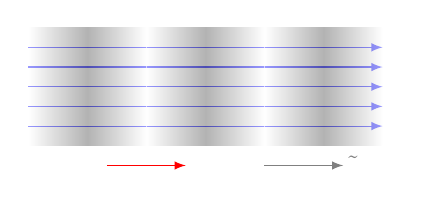
\begin{tikzpicture}[>=latex]
    \foreach[count=\c] \y in {0,0.25,...,1} {
        \draw[blue, ->] (0, \y) -- ++(4.5, 0) \ifnum\c=3 node[right] {$\B$} \fi;
%        \draw[red, thick, ->] (0.5, \y) -- ++(0.5, 0);
%        \draw[red, thick, ->] (2, \y) -- ++(-0.5, 0);
%        \draw[red, thick, ->] (2.5, \y) -- ++(0.5, 0);
%        \draw[red, thick, ->] (4, \y) -- ++(-0.5, 0);
    }
    \foreach \x in {0,0.75,1.5}{
     \begin{scope}[shift={(\x, 0)}]
\path[left color=white,right color=white,middle color=gray, opacity=0.6] (\x, -0.25) rectangle ++(1.5, 1.5);
\end{scope}
    }

    \draw[red, ->] (1, -0.5) -- (2, -0.5) node[right] {$\wk$};
    \draw[gray, ->] (3, -0.5) -- (4, -0.5) node[right] {$\tilde{\V}$};

\end{tikzpicture}
	\end{center}
	\begin{block}{}\justifying
		Магнітне поле <<вморожене>> в плазму і при стиснені середовища вздовж магнітного поля густина речовини буде змінюватись, а$\B = \const$. Хвиля виникає за рахунок зміни густини середовища --- зміни густини іонів --- це звукова хвиля, швидкість якої:
		\begin{equation*}
			c_s = \sqrt{\left(\frac{dp}{d\rho}\right)_{S=\const}} = \sqrt{\gamma\frac{p_0}{Mn_0}},
		\end{equation*}
	\end{block}
\end{frame}
% ===========================================================================

% ============================== Слайд ## ===================================
\begin{frame}{Магнітний звук}{Якісний розгляд}
	\begin{block}{}
		Розглянемо збурення $\tilde{\V}_\perp$, що поширюється поперек напрямку магнітного поля $\wk \perp \B$, $\tilde{\V} \parallel \wk$:
		\begin{equation*}
			\tilde{\V}_\perp = \tilde{\V}_m e^{-i(\omega t - k_xx - k_yy)}.
		\end{equation*}
	\end{block}
	\begin{center}
		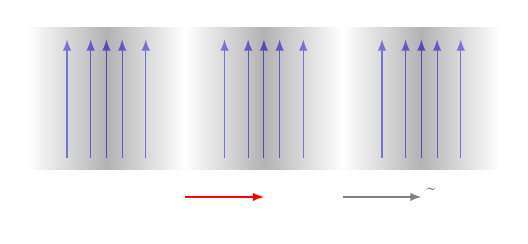
\begin{tikzpicture}[>=latex]
    \def\h{1.5}
    \foreach[count=\c] \x in {0,2,...,4} {

\begin{scope}[shift={(\x, 0)}]
        \draw[blue, ->] (-0.5,0) -- ++(0, \h);
        \draw[blue, ->] (-0.2,0) -- ++(0, \h);
        \draw[blue, ->] (0,0) -- ++(0, \h);
        \draw[blue, ->] (+0.2,0) -- ++(0, \h);
        \draw[blue, ->] (+0.5,0) -- ++(0, \h);
        \path[left color=white,right color=white,middle color=gray, opacity=0.6] (-1, -0.15) rectangle ++(2, {\h + 0.3});
\end{scope}
    }
\draw[red, ->] (1, -0.5) -- (2, -0.5) node[right] {$\wk$};
\draw[gray, ->] (3, -0.5) -- (4, -0.5) node[right] {$\tilde{\V}$};
\end{tikzpicture}
	\end{center}
	\begin{onlyenv}<1>
		\begin{block}{}\justifying
			При стиснені середовища поперек магнітного поля густина речовини буде змінюватись разом з магнітним полем $\B = C\rho$. Ця хвиля є магнітнозвуковою хвилею, швидкість якої:
			\begin{equation*}
				c = \sqrt{\left(\frac{dp}{d\rho}\right)_{S=\const}} = \sqrt{\gamma\frac{p_0}{Mn_0} + \frac{B^2}{4\pi Mn_0}} = \sqrt{c_s^2 + c_A^2}.
			\end{equation*}
		\end{block}
        \end{onlyenv}
		\begin{onlyenv}<2>
		\begin{block}{}
			Альвенівська швидкість:
			\begin{equation*}
				\tcbhighmath{
					c_A = \frac{B}{\sqrt{4\pi\rho}}.
				}
			\end{equation*}
		\end{block}
	\end{onlyenv}
\end{frame}
% ===========================================================================

% ============================== Слайд ## ===================================
\begin{frame}{Альвенівські хвилі}{}
	\begin{block}{}
		Альвенівські хвилі --- поперечні магнітогідродинамічні плазмові хвилі, що поширюються вздовж силових ліній магнітного поля  ($\wk \parallel \B$, $\tilde{\V} \perp \wk$).
		\begin{equation*}
			\tilde{\V}_\perp = \tilde{\V}_m e^{-i(\omega t - k_zz)}.
		\end{equation*}
	\end{block}
	\begin{center}
		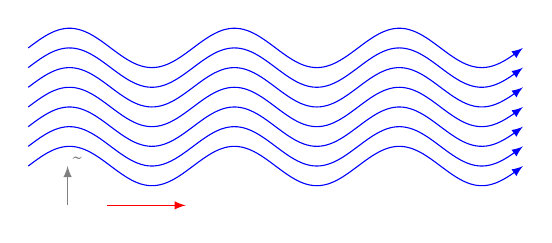
\begin{tikzpicture}[>=latex]
    \foreach \shift in {0,...,6} {
    \draw[->, blue, domain=0:2*pi, samples=150] plot ({\x}, {0.25*\shift + 0.25*sin(3*\x r)});
    }
    \draw[red, ->] (1, -0.5) -- (2, -0.5) node[right] {$\wk$};
    \draw[gray, ->] (0.5, -0.5) -- ++(0, 0.5) node[right] {$\tilde{\V}$};
\end{tikzpicture}
	\end{center}
	\begin{block}{}\justifying
		Хвиля подібна до поперечних хвиль на струні (магнітні силові лінії поводять себе як пружні нитки). В ролі сили натягу  виступає величина $B_0^2/4\pi$.  Оскільки віддаль між сусідніми магнітними силовими лініями не змінюється --- альвенівські хвилі не збурюють густину плазми. Відповідно пружні властивості середовища для цих хвиль визначаються лише магнітним полем.
	\end{block}
\end{frame}
% ===========================================================================

% ============================== Слайд ## ===================================
\begin{frame}{Лінеаризація рівнянь гідродинаміки}{}
	\begin{onlyenv}<1>
		\begin{block}{}\justifying


			Будемо користуватися моделлю однорідинної гідродинаміки.
			\begin{align*}
				Mn_0 \left(\dt{\V} + \scdot\V\nabla \V\right) & = - \grad{p} + \frac1{4\pi}\vecdot{(\rot{\B})}{\B}, \\
				\dt{n} + \divg{(n\V)}                         & = 0,                                                \\
				\dt{\B}                                       & = \rot{\vecdot{\V}{\B}}.
			\end{align*}

			Ці рівняння розв'язуються, застосовуючи \alert{процедуру лінеаризації}, яка що амплітуда коливань
			вважається малою, і тому членами, що містять високі степені амплітуд, нехтують:

			\begin{equation*}
				n = n_0 + n,  \quad p = p_0 + \tilde{p}, \quad B  = B_0 + \tilde{B}, \quad \V =  \tilde{\V}.
			\end{equation*}
		\end{block}
	\end{onlyenv}
	\begin{onlyenv}<2>
		\begin{align*}
			Mn_0 \dt{\V} &+ c_s^2\grad{M\tilde{n}}   + \frac1{4\pi}\vecdot{\B_0}{(\rot{\tilde{\B}})} = 0, \\
			\dt{\tilde{n}} &+ n_0 \divg{\tilde{\V}}  = 0,                                                                  \\
			\dt{\tilde{\B}}                        & = \rot{\vecdot{\tilde{\V}}{\B_0}}.
		\end{align*}
		Ці рівняння можна привести до одного рівняння відносно змінної $\tilde{\V}$:
		% Продиференціюємо рівняння руху за часом
		\begin{equation*}
			\ddt{\tilde{\V}} - c_s^2\grad{(\divg{\tilde{\V})}} +
			\vec{c}_A\times\left[\rot{\left[\rot{\vecdot{\tilde{\V}}{\vec{c}_A}}\right]}\right] = 0.
		\end{equation*}
	\end{onlyenv}
\end{frame}
% ===========================================================================

% ============================== Слайд ## ===================================
\begin{frame}{Плоскі хвилі}{}
	Розв'язок представним у вигляді плоских хвиль:
	\begin{equation*}
		\tilde{\V}(\vec{r}, t) = \tilde{\V}e^{i\scdot{\wk}{\vec{r}} - i\omega t}.
	\end{equation*}
	\begin{multline*}
		%
		-\omega^2\tilde{\V} + (c_s^2 + c_A^2)\scdot{\wk}{\tilde{\V}}\wk + \\
		\scdot{\wk}{\vec{c}_A}\left[\scdot{\wk}{\vec{c}_A}\tilde{\V} - \scdot{\vec{c}_A}{\tilde{\V}}\wk - \scdot{\wk}{\tilde{\V}}\vec{c}_A  \right] = 0.
	\end{multline*}
\end{frame}

\begin{frame}{Магнітозвукова хвиля}{Поширення перпендирулярно до магнітного поля}
	\begin{onlyenv}<1>
		\begin{block}{}\justifying
			У випадку $\wk\perp \B$: \(\scdot{\wk}{\B_0} = 0\) або \(\scdot{\wk}{\vec{c}_A} = 0 \).

			Рівняння зводиться до виразу:
			\begin{equation*}
				-\omega^2\tilde{\V} + (c_s^2 + c_A^2)\scdot{\wk}{\tilde{\V}}\wk = 0,
			\end{equation*}
			звідки
			\begin{equation*}
				\tilde{\V} = \frac1{\omega^2}(c_s^2 + c_A^2)\scdot{\wk}{\tilde{\V}}\wk.
			\end{equation*}
			Якщо $\tilde{\V}\parallel\wk$ ---  розв'язок для $\tilde{\V}$ дає поздовжню хвилю з фазовою швидкістю:
			\begin{equation*}
				\frac\omega{k} = \sqrt{c_s^2 + c_A^2}.
			\end{equation*}
			Це поздовжня хвиля: коливання швидкості (і густини) спрямовані в напрямку поширення хвилі. Тому цю хвилю було названо \alert{магнітозвуковою хвилею}.
		\end{block}
	\end{onlyenv}
	\begin{onlyenv}<2>
		\begin{block}{}\justifying
			Магнітне поле, пов'язане з цією поздовжньою хвилею:
			\begin{equation*}
				\tilde{\B}(\vec{r}, t) = \tilde{\B}e^{i\scdot{\wk}{\vec{r}} - i\omega t},
			\end{equation*}
			з рівняння вмороженого поля
			\begin{equation*}
				-\omega\tilde{\B} - \vecdot{\wk}{\vecdot{\tilde{\V}}{\B_0}} = 0.
			\end{equation*}
			звідки
			\begin{equation*}
				\tilde{\B} = \frac{\tilde{v}}{\omega / k} \B_0, \quad \E = -\frac1c\vecdot{\tilde{\V}}{\B_0}.
			\end{equation*}

			Ця хвиля схожа до електромагнітної хвилі (але поздовжня):
			\begin{itemize}
				\item змінне магнітне поле перпендикулярне до напрямку поширення, але паралельне магнітостатичному полю;
				\item електричне поле перпендикулярне як напряму поширення, так і магнітостатичному полю.
			\end{itemize}
		\end{block}
	\end{onlyenv}
	\framesubtitle<3>{Властивості}
	\begin{onlyenv}<3>
		\begin{itemize}\justifying
			\item Фазова швидкість не залежить від частоти, отже \alert{хвиля недиспергуюча}.
			\item Під час поширення хвиля створює області стиснення і розрідження в
			      магнітних силових лініях, але не \alert{змінює напрямку магнітного поля}.
			\item Лінії магнітного поля і рідина \alert{рухаються разом}.
			\item Якщо $p \gg \frac{B^2}{8\pi}$ --- вплив магнітних силових ліній нехтувано малий, тому $\omega/k = c_s$ і хвиля стає звичайною звуковою хвилею.
			\item Якщо $p \ll \frac{B^2}{8\pi}$ --- фазова швидкість магнітозвукової хвилі стає рівною альвенівській швидкості.

			      {\scriptsize  Ця мода магнітозвукової хвилі також відома як \alert{альвенівська хвиля стиснення} або \alert{швидка альвенівська хвиля} (швидка магнітозвукова хвиля). }
		\end{itemize}
	\end{onlyenv}
\end{frame}
% ===========================================================================

% ============================== Слайд ## ===================================
\begin{frame}{Альвенівська хвиля}{Поширення паралельно до магнітного поля}
	\begin{block}{}\justifying
		У випадку $\wk\parallel \B_0$: \(\scdot{\wk}{\vec{c}_A} = kc_A \):
		\begin{equation*}
			(k^2c_A^2 - \omega^2)\tilde{\V} + \left( 1 - \frac{c_s^2}{c_A^2}\right) k^2\scdot{\tilde{\V}}{\vec{c}_A}\vec{c}_A = 0.
		\end{equation*}
\begin{overprint}
\onslide<1>
		При $\tilde{\V} \parallel \B_0$ та $\tilde{\V} \parallel \wk$ можлива поздовжня мода з фазовою швидкістю:
		\begin{equation*}
			\omega/k = c_s.
		\end{equation*}
		Це звичайна поздовжня звукова хвиля, що поширюється в напрямку руху плазми. З цією хвилею не пов'язане ні електричне поле, ні густина електричного струму, ні магнітне поле.
\onslide<2>
При $\tilde{\V} \perp \B_0$ та $\tilde{\V} \perp \wk $ ($\wk \parallel \B_0$): $\scdot{\tilde{\V}}{\vec{c}_A} = 0$ фазова швидкість хвилі:
\begin{equation*}
    \omega/k = c_A.
\end{equation*}
 Ця поперечна хвиля називається \alert{альвенівська хвиля зсуву} або \alert{повільна альфвенівська хвиля} (або просто \alert{альвенівська} хвиля).  Дисперсія відсутня.

\onslide<3>

Магнітне поле, пов'язане з цією хвилею, задається таким виразом:
\begin{equation*}
    \tilde{\B} = -\frac{B_0}{\omega / k}\tilde{\V}.
\end{equation*}
Магнітне поле збурення перпендикулярне початвовому полю $\tilde{\B} \perp \B_0$.

Альвенівська хвиля не призводить до коливань густини рідини або тиску, хоча і лінії струму, і магнітні силові лінії осцилюють у площині, перпендикулярній до $\B_0$.


\end{overprint}
	\end{block}
\end{frame}
% ===========================================================================

% ============================== Слайд ## ===================================
%\begin{frame}{Діаграми хвильової нормалі}{}
%       \begin{block}{}\justifying
%    Залежність фазової швидкості від кута між векторами $\wk$ та $\B_0$ для хвиль зручно представляти за допомогою діаграми поверхонь фазової швидкості (поверхонь хвильової нормалі), які показують залежність довжини вектора фазової швидкості від напрямку магнітного поля.
%\end{block}
%\begin{center}
%
\tikzset{
    legend/.style= {right, font=\scriptsize, inner sep=0},
    declare function = {
    xmax=4;
    ymax=4;
    fast(\x)  = 1/sqrt(2) * sqrt( (cs^2 + cA^2) + sqrt(  (cs^2 + cA^2)^2 - 4 * cs^2*cA^2*(cos(\x))^2 ) );
    slow(\x)  = 1/sqrt(2) * sqrt( (cs^2 + cA^2) - sqrt(  (cs^2 + cA^2)^2 - 4 * cs^2*cA^2*(cos(\x))^2 ) );
    alven(\x) = cA*cos(\x);
    }
}

\colorlet{alven}{green!60!black}
\colorlet{slow}{red}
\colorlet{fast}{blue}

\begin{tikzpicture}[>=latex,
declare function={
    cs=3;
    cA=2.25;
},
]
    %Легенда
    \draw[fast] (1, {ymax-0.25}) -- ++(0.25,0) node[legend] {Швидка хвиля};
    \draw[slow] (1, {ymax-0.5}) -- ++(0.25,0) node[legend] {Повільна хвиля};
    \draw[alven] (1, {ymax-0.75}) -- ++(0.25,0) node[legend] {Альвенівська хвиля};

    \draw[->] (0, 0) -- ++(0, ymax);
    \draw[->, blue] (-0.5, 0.5) -- ++(0, 1) node[left] {$\vec{B}_0$};
    \draw[->] (0, 0) -- ++(xmax, 0);
    \draw [thick,color=alven,domain=0:90,samples=200,smooth]  plot ({\x}:{alven(90-\x)});
    \draw [thick,color=slow,domain=0:90,samples=200,smooth]  plot ({\x}:{slow(90-\x)});
    \draw [thick,color=fast,domain=0:90,samples=300,smooth]  plot ({\x}:{fast(90-\x)});

   \pgfmathsetmacro\a{55}

    \draw[alven, ->] (0,0) -- (\a:{alven(90-\a)});
    \draw[slow, ->] (0,0) -- (\a:{slow(90-\a)});
    \draw[fast, ->] (0,0) -- (\a:{fast(90-\a)});


    \draw (0,0.5) arc(90:\a:0.5) node[pos=0.5, anchor=south] {$\theta$};

    \node[left] at (0, {slow(0)}) {$c_A$};
    \node[left] at (0, {fast(0)}) {$c_s$};
    \node[below left, font=\scriptsize] at ({fast(90)}, 0) {$\sqrt{c_A^2 + c_s^2}$};
\end{tikzpicture}
%
\begin{tikzpicture}[>=latex,
declare function={
    cs=2.25;
    cA=3;
},
]

    %Легенда
    \draw[fast] (1, {ymax-0.25}) -- ++(0.25,0) node[legend] {Швидка хвиля};
    \draw[slow] (1, {ymax-0.5}) -- ++(0.25,0) node[legend] {Повільна хвиля};
    \draw[alven] (1, {ymax-0.75}) -- ++(0.25,0) node[legend] {Альвенівська хвиля};

    \draw[->] (0, 0) -- ++(0, ymax);
    \draw[->, blue] (-0.5, 0.5) -- ++(0, 1) node[left] {$\vec{B}_0$};
    \draw[->] (0, 0) -- ++(xmax, 0);
    \draw [thick,color=alven,domain=0:90,samples=200,smooth]  plot ({\x}:{alven(90-\x)});
    \draw [thick,color=slow,domain=0:90,samples=200,smooth]  plot ({\x}:{slow(90-\x)});
    \draw [thick,color=fast,domain=0:90,samples=300,smooth]  plot ({\x}:{fast(90-\x)});

    \pgfmathsetmacro\a{45}

    \draw[fast, ->] (0,0) -- (\a:{fast(90-\a)});
    \draw[alven, ->] (0,0) -- (\a:{alven(90-\a)});
    \draw[slow, ->] (0,0) -- (\a:{slow(90-\a)});

    \draw (0,0.5) arc(90:\a:0.5) node[pos=0.5, anchor=south] {$\theta$};
    \node[left] at (0, {slow(0)}) {$c_s$};
    \node[left] at (0, {fast(0)}) {$c_A$};
    \node[below left, font=\scriptsize] at ({fast(90)}, 0) {$\sqrt{c_A^2 + c_s^2}$};
\end{tikzpicture}
%\end{center}
%\end{frame}
% ===========================================================================

% ============================== Слайд ## ===================================
\begin{frame}{Задачі}{}
       \begin{exampleblock}{Задача 1}\justifying
    Обчислити швидкість альфвенівської хвилі для таких випадків:
\begin{enumerate}
\item Іоносфера Землі, припускаючи $n_e = 10^7$ м\textsuperscript{-3} і $B = 10^{-3}$~Гс. Переносники позитивного заряду --- іони атомів кисню.
\item Сонячна корона, припускаючи $n_e = 10^6$ см\textsuperscript{-3} і $B = 10$~Гс. Переносники позитивного заряду --- протони.
\item Міжзоряний простір, припускаючи  $n_e = 10^7$ м\textsubscript{-3} і $B = 10^{-3}$~Гс. Переносники позитивного заряду --- протони.
\end{enumerate}
\end{exampleblock}
\begin{exampleblock}{Задача 2}\justifying
Врахувати ефект скінченної провідності під час виведення рівнянь
для плоскої альвенівської хвилі, що поширюється вздовж
магнітного поля. Показати, що розв'язки виду $\exp(\alpha x - i\omega t)$ задовольняють
лінеаризованим рівнянням. Знайдіть вираз для коефіцієнту $\alpha$.
\end{exampleblock}
\end{frame}
% ===========================================================================

% ============================== Слайд ## ===================================
\begin{frame}{Задачі}{}
       \begin{exampleblock}{Задача 3}
%  Нехай $\tilde{v}_{\ell}$ і $\tilde{v}_t$ (індекси $\ell$ і $t$ не плутати з $\perp$ і $\parallel$) позначають поздовжню і поперечну
%компоненти масової швидкості потоку до напрямку поширення $\wk$ для
%швидкої та повільної МГД-хвиль. Показати, що щ і щ перебувають
%у фазі для швидкої хвилі та у протифазі 180° для повільної хвилі.
%Також показати, що збурення кінетичного та магнітного тисків
%перебувають у фазі для швидкої хвилі й у протифазі для повільної
%хвилі.
Дослідіть випадок поширення хвиль в довільному напрямку відносно вектора магнітної індукції $\B_0$ (слайд 9). Покажіть, що закон дисперсії для
\emph{магнітозвукових} хвиль має вигляд:
\begin{equation*}\justifying
    \left(\frac{\omega}{k}\right)^2 = \frac12\left( c^s_s + c^2_A \right) \pm \frac12\left[ \left( c^s_s + c^2_A \right)^2 -
    4c_s^2c_A^2\cos^2\theta\right]^{1/2}.
\end{equation*}

Розв'язки зі знаками <<$+$>> і <<$-$>> називаються відповідно \textit{швидкою} і \textit{повільною} магнітозвуковими хвилями .

\bigskip

\textit{Вказівка}: Без втрати загальності можна ввести декартову систему координат, у якій вісь $y$
перпендикулярна площині, заданій хвильовим вектором $\wk$ і вектором магнітної індукції $\B_0$, а вісь
$z$ паралельна $\B_0$. Введіть кут $\theta$: $\scdot{\wk}{\B_0} = kB_0\cos\theta$. Тобто, вектор $\wk$ можна представити як:
\begin{equation*}
    \wk = k(\vec{e}_x\sin\theta + \vec{e}_z\cos\theta),
\end{equation*}
а $\tilde{\V}$ як:
\begin{equation*}
    \tilde{\V} = \tilde{v}_x\vec{e}_x + \tilde{v}_y\vec{e}_y+ \tilde{v}_y\vec{e}_y.
\end{equation*}

\end{exampleblock}
\end{frame}
% ===========================================================================

\end{document}

